\emph{Project planning} is typically a in iterative process that starts
at project initiation and continues evolving. In order to set up a
suitable \emph{project schedule}, and in particular decide the time
and resource allocation, we need to identify:
\begin{itemize}
\item \emph{tasks}: activities that must be completed to achieve the project
goal and the corresponding dependencies;
\item \emph{milestones}: points in time in which you can assess the progress
of the project;
\item \emph{deliverables}: work products delivered to the stakeholders.
\end{itemize}
This phase has to be driven by the \emph{software development process}
chosen and by the main features of the specific application we are
going to design. In this section we provide a description of the tasks,
their dependencies and a graphical representation of a schedule proposal.


\subsection{Tasks}

The following schedule tries to be a compromise between the need of
producing a realistic program of the tasks and be compatible with
the tasks we really performed during the semester. For what concerns
the tasks related to RASD, DD and ITDP the dates are the real ones,
for PP we assumed to having performed it as the first activity (as
it is in a realistic context). Since we didn't perform the implementation
of the software we couldn't exploit real data; to be realistic we
allocate a duration of about three months. Also for code inspection
and testing we choose reasonable duration. We can interpret this program
as a schedule for an hypothetical annual project assigned to us at
the beginning of the academic year. We didn't use the duration value
provided by COCOMO II analysis since, also according to the applications
made in the examples by the previous years, it tends to overestimate
project duration and not to be coherent with the ``breakneck speed''
we are asked to keep at Politecnico.

\newpage{}

The following table shows for each task the id, name, star and end
date, the duration expressed in working days and the possible precedences.
Task are grouped into macro tasks.

\noindent \begin{center}
\begin{tabular}{l|>{\raggedright}p{4cm}|l|l|r|l}
\hline 
\emph{Task id} & \emph{Name} & \emph{Start} & \emph{End} & \emph{Duration} & \emph{Precendences}\tabularnewline
\hline 
\hline 
T1 & \textbf{Project planning} & 01/10/2015 & 14/10/2015 & 10 & -\tabularnewline
\hline 
T11 & {\footnotesize{}Project scheduling} & {\footnotesize{}01/10/2015} & {\footnotesize{}09/10/2015} & {\footnotesize{}7} & -\tabularnewline
\hline 
T12 & {\footnotesize{}Resource allocation} & {\footnotesize{}12/10/2015} & {\footnotesize{}14/10/2015} & {\footnotesize{}3} & T11\tabularnewline
\hline 
T13 & {\footnotesize{}Risk planning} & {\footnotesize{}05/10/2015} & {\footnotesize{}14/10/2015} & {\footnotesize{}8} & -\tabularnewline
\hline 
M1 & \textcolor{red}{PP} & \textcolor{red}{15/10/2015} & \textcolor{red}{15/10/2015} & \textcolor{red}{-} & \tabularnewline
\hline 
T2 & \textbf{Requirement analysis and specification} & \textbf{15/10/2015} & \textbf{02/11/2015} & \textbf{13} & M1\tabularnewline
\hline 
T21 & {\footnotesize{}Requirement engineering} & {\footnotesize{}15/10/2015} & {\footnotesize{}21/10/2015} & {\footnotesize{}5} & \tabularnewline
\hline 
T22 & {\footnotesize{}Use case design} & {\footnotesize{}22/10/2015} & {\footnotesize{}02/11/2015} & {\footnotesize{}8} & T22\tabularnewline
\hline 
T23 & {\footnotesize{}High level data design} & {\footnotesize{}26/10/2015} & {\footnotesize{}28/10/2015} & {\footnotesize{}3} & \tabularnewline
\hline 
T24 & {\footnotesize{}Alloy modeling} & {\footnotesize{}29/10/2015} & {\footnotesize{}02/11/2015} & {\footnotesize{}3} & T23\tabularnewline
\hline 
M2 & \textcolor{red}{RASD} & \textcolor{red}{03/11/2015} & \textcolor{red}{03/11/2015} & \textcolor{red}{-} & \tabularnewline
\hline 
T3 & \textbf{Acceptance test plan design} & \textbf{03/11/2015} & \textbf{11/11/2015} & \textbf{7} & M2\tabularnewline
\hline 
T4 & \textbf{Design} & \textbf{09/11/2015} & \textbf{04/12/2015} & \textbf{20} & M2\tabularnewline
\hline 
T41 & {\footnotesize{}Architectural design} & {\footnotesize{}09/11/2015} & {\footnotesize{}04/12/2015} & {\footnotesize{}20} & \tabularnewline
\hline 
T42 & {\footnotesize{}Algorithm design} & {\footnotesize{}16/11/2015} & {\footnotesize{}04/12/2015} & {\footnotesize{}15} & \tabularnewline
\hline 
T43 & {\footnotesize{}User interface design} & {\footnotesize{}30/11/2015} & {\footnotesize{}04/12/2015} & {\footnotesize{}5} & \tabularnewline
\hline 
M3 & \textcolor{red}{DD} & \textcolor{red}{07/12/2015} & \textcolor{red}{07/12/2015} & \textcolor{red}{-} & \tabularnewline
\hline 
T5 & \textbf{Unit test plan design} & \textbf{07/12/2015} & \textbf{15/12/2015} & \textbf{7} & M2\tabularnewline
\hline 
T6 & \textbf{Integration test plan design} & \textbf{07/01/2016} & \textbf{21/01/2016} & \textbf{11} & M2\tabularnewline
\hline 
M4 & \textcolor{red}{ITDP} & \textcolor{red}{22/01/2016} & \textcolor{red}{22/01/2016} & \textcolor{red}{-} & \tabularnewline
\hline 
T7 & \textbf{Implementation} & \textbf{07/12/2015} & \textbf{05/03/2016} & \textbf{65} & M2\tabularnewline
\hline 
T71 & {\footnotesize{}Components implementation} & {\footnotesize{}07/12/2015} & {\footnotesize{}05/03/2016} & {\footnotesize{}65} & \tabularnewline
\hline 
T72 & {\footnotesize{}Subsystem implementation} & {\footnotesize{}08/02/2016} & {\footnotesize{}04/03/2016} & {\footnotesize{}20} & \tabularnewline
\hline 
T8 & \textbf{Code Inspection} & \textbf{07/03/2016} & \textbf{23/03/2016} & \textbf{13} & \tabularnewline
\hline 
T81 & {\footnotesize{}Manual inspection} & {\footnotesize{}07/03/2016} & {\footnotesize{}17/03/2016} & {\footnotesize{}9} & T71\tabularnewline
\hline 
T82 & {\footnotesize{}Automated code inspection} & {\footnotesize{}18/03/2016} & {\footnotesize{}23/03/2016} & {\footnotesize{}4} & T81\tabularnewline
\hline 
M5 & \textcolor{red}{CI} & \textcolor{red}{24/03/2016} & \textcolor{red}{24/03/2016} & \textcolor{red}{-} & \tabularnewline
\hline 
T9 & \textbf{Testing} & \textbf{24/03/2016} & \textbf{28/04/2016} & \textbf{26} & \tabularnewline
\hline 
T91 & {\footnotesize{}Unit testing} & {\footnotesize{}24/03/2016} & {\footnotesize{}08/04/2016} & {\footnotesize{}12} & T5, T71\tabularnewline
\hline 
T92 & {\footnotesize{}Integration testing} & {\footnotesize{}11/04/2016} & {\footnotesize{}18/04/2016} & {\footnotesize{}6} & T91, T6, T7\tabularnewline
\hline 
T93 & {\footnotesize{}System and performance testing} & {\footnotesize{}19/04/2016} & {\footnotesize{}20/04/2016} & {\footnotesize{}2} & T92\tabularnewline
\hline 
T94 & {\footnotesize{}Acceptance testing} & {\footnotesize{}21/04/2016} & {\footnotesize{}28/04/2016} & {\footnotesize{}6} & T93, T3\tabularnewline
\hline 
T10 & \textbf{Deployment} & \textbf{29/04/2016} & \textbf{04/05/2016} & \textbf{4} & T9\tabularnewline
\hline 
\end{tabular}
\par\end{center}

\medskip{}


\newpage{}

The following is the same table in which just macro tasks and the
delivarables are represented.

\noindent \begin{center}
\begin{tabular}{l|>{\raggedright}p{4cm}|l|l|r}
\hline 
\emph{Task id} & \emph{Name} & \emph{Start} & \emph{End} & \emph{Duration}\tabularnewline
\hline 
\hline 
T1 & \textbf{Project planning} & 01/10/2015 & 14/10/2015 & 10\tabularnewline
\hline 
M1 & \textcolor{red}{PP} & \textcolor{red}{15/10/2015} & \textcolor{red}{15/10/2015} & \textcolor{red}{-}\tabularnewline
\hline 
T2 & \textbf{Requirement analysis and specification} & \textbf{15/10/2015} & \textbf{02/11/2015} & \textbf{13}\tabularnewline
\hline 
M2 & \textcolor{red}{RASD} & \textcolor{red}{03/11/2015} & \textcolor{red}{03/11/2015} & \textcolor{red}{-}\tabularnewline
\hline 
T3 & \textbf{Acceptance test plan design} & \textbf{03/11/2015} & \textbf{11/11/2015} & \textbf{7}\tabularnewline
\hline 
T4 & \textbf{Design} & \textbf{09/11/2015} & \textbf{04/12/2015} & \textbf{20}\tabularnewline
\hline 
M3 & \textcolor{red}{DD} & \textcolor{red}{07/12/2015} & \textcolor{red}{07/12/2015} & \textcolor{red}{-}\tabularnewline
\hline 
T5 & \textbf{Unit test plan design} & \textbf{07/12/2015} & \textbf{15/12/2015} & \textbf{7}\tabularnewline
\hline 
T6 & \textbf{Integration test plan design} & \textbf{07/01/2016} & \textbf{21/01/2016} & \textbf{11}\tabularnewline
\hline 
M4 & \textcolor{red}{ITDP} & \textcolor{red}{22/01/2016} & \textcolor{red}{22/01/2016} & \textcolor{red}{-}\tabularnewline
\hline 
T7 & \textbf{Implementation} & \textbf{07/12/2015} & \textbf{05/03/2016} & \textbf{65}\tabularnewline
\hline 
T8 & \textbf{Code Inspection} & \textbf{07/03/2016} & \textbf{23/03/2016} & \textbf{13}\tabularnewline
\hline 
M5 & \textcolor{red}{CI} & \textcolor{red}{24/03/2016} & \textcolor{red}{24/03/2016} & \textcolor{red}{-}\tabularnewline
\hline 
T9 & \textbf{Testing} & \textbf{24/03/2016} & \textbf{28/04/2016} & \textbf{26}\tabularnewline
\hline 
T10 & \textbf{Deployment} & \textbf{29/04/2016} & \textbf{04/05/2016} & \textbf{4}\tabularnewline
\hline 
\end{tabular}
\par\end{center}


\subsection{Milestones}

Here are the expected milestone of the project.
\begin{enumerate}
\item after RASD
\item after DD
\item after CI
\item after implementation
\item after testing
\item after deployment
\end{enumerate}

\subsection{Deliverables}

Here are the expected deliverables of the project; the ones we really
produced in the semester are highlighted in red in the previous table
(actually we didn't perform code inspection on the myTaxiService but
we included it as a deliverable anyway).
\begin{enumerate}
\item RASD (Requirement Analysis and Specification Document) 
\item DD (Design Document)
\item CI (Code Inspection Report)
\item Code
\item UTPD (Unit Test Design Plan)
\item ITPD (Integration Test Design Plan)
\item User manual
\end{enumerate}
\begin{landscape}

\newgeometry{left=-7cm,bottom=0cm,top=2.5cm,right=2cm}


\subsection{Gantt chart}

\medskip{}


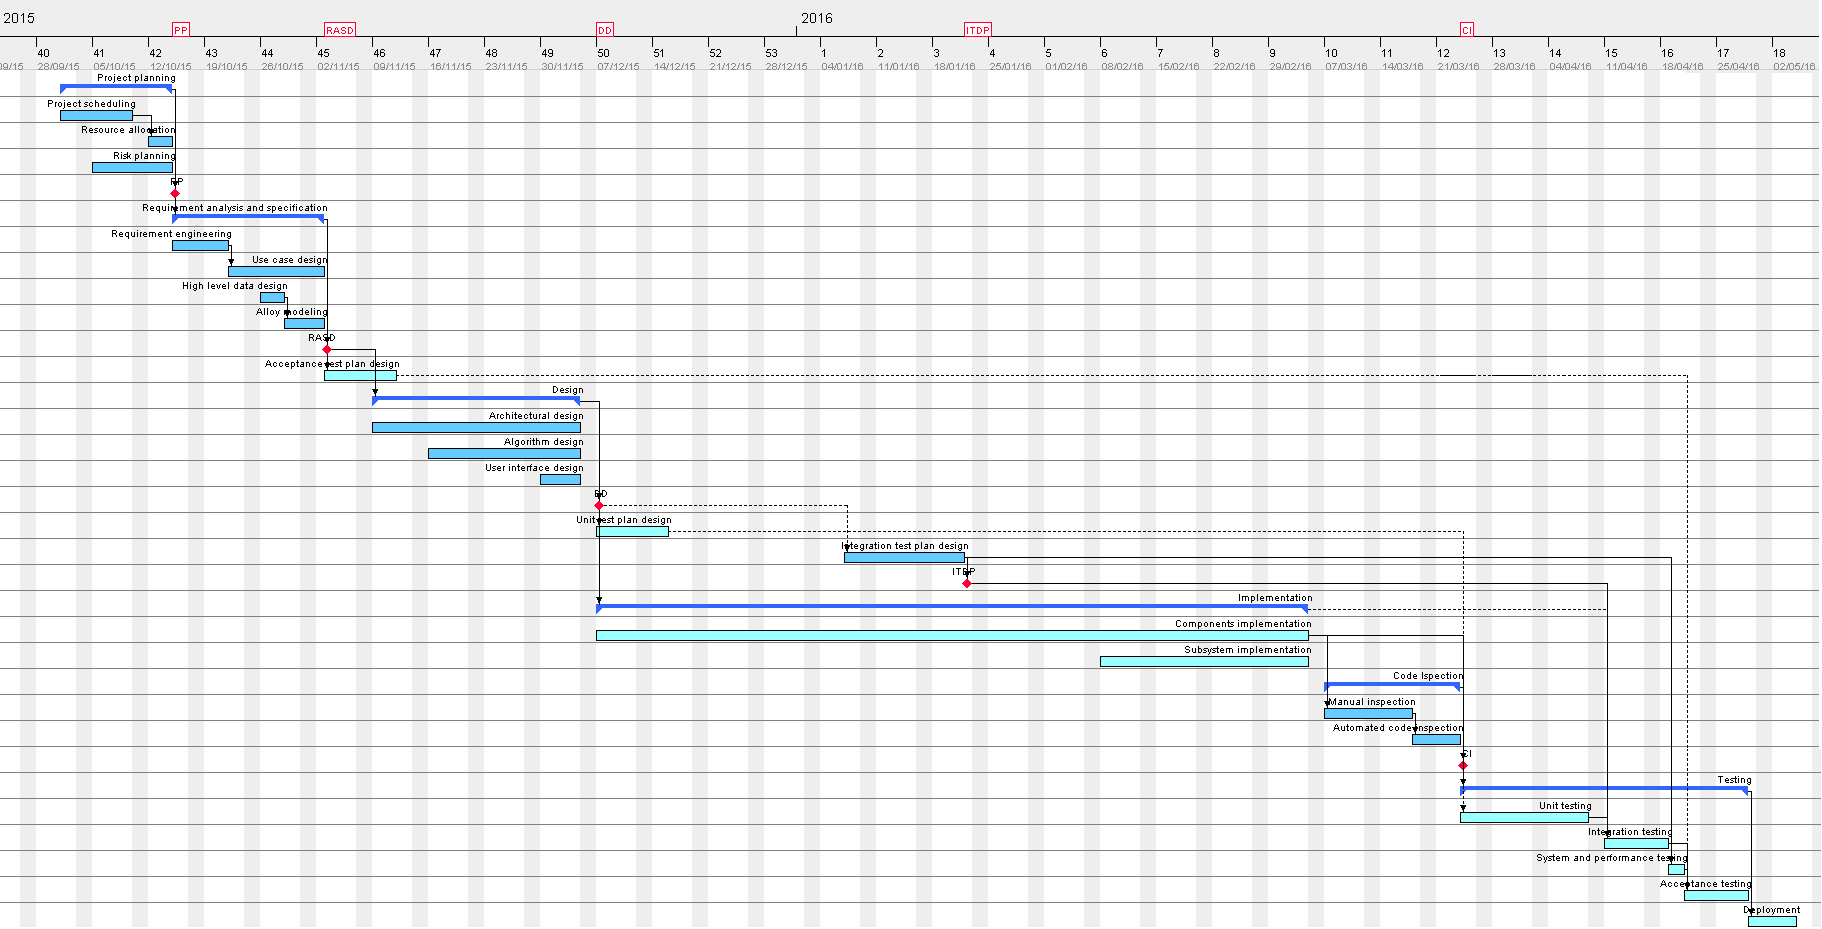
\includegraphics[scale=0.53]{tasks/gantt}

\restoregeometry

\end{landscape}
